\chapter{Обзор существующих подходов и теоретическая справка}
\label{cha:ch_1}


\section{Архитектуры нейронных сетей для синтеза речи}
Современные решения для преобразования текста в речь в основном устроены следующим образом: (cм. Рисунок \ref{fig:tts_pipeline})

\begin{enumerate}
    \item В начале текст токенизируется - преобразуется из строкового формата в последовательность лексем - токенов
    \item токенизированный текст преобразуется с помощью нейросети-энкодера во внутреннее признаковое представление
    \item используя текстовые признаки, нейросеть генерирует признаковое представление звука или спектрограмму. Этот модуль может быть многоуровненвым и сложным в зависимости от архитектуры.
    \item признакове представление звука декодируется в звуковой сигнал.
\end{enumerate}

\begin{figure}[t]
  \centering
  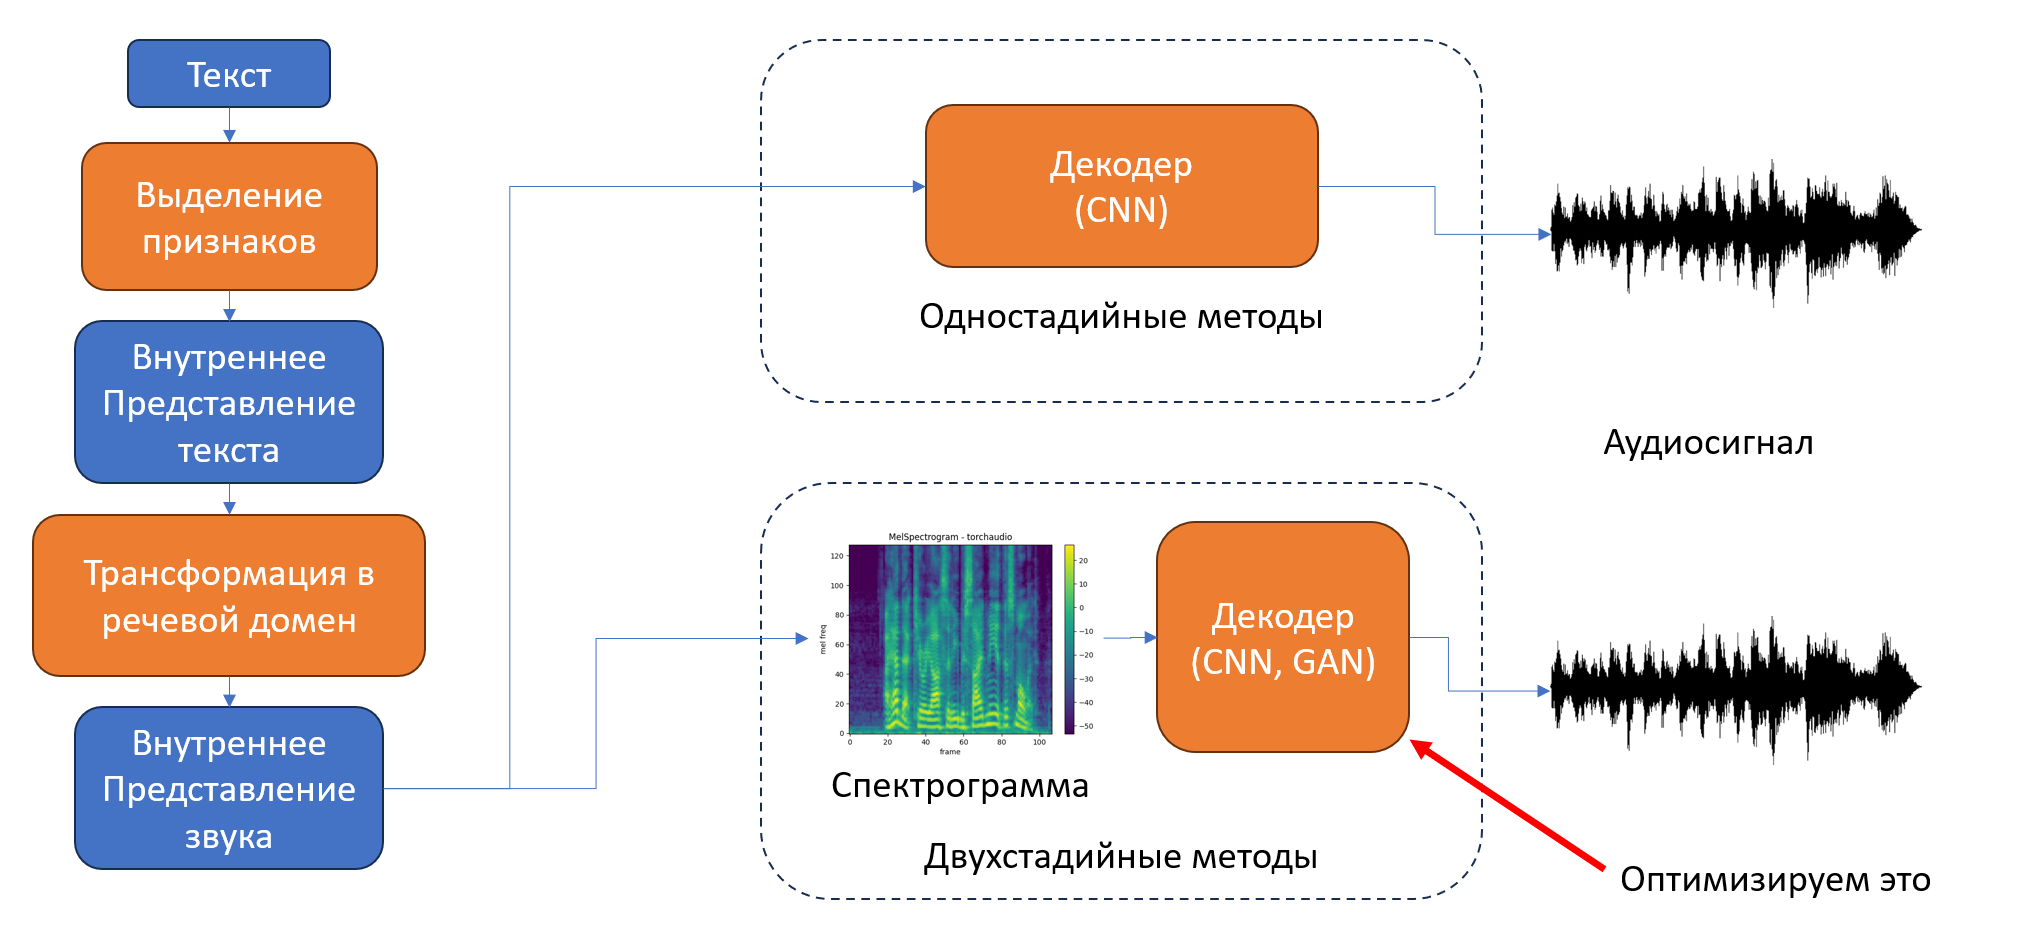
\includegraphics[width=16cm]{figures/tts_pipeline}
  \caption{Преобразование текста в речь}
  \label{fig:tts_pipeline}
\end{figure}

Также помимо задачи преобразования текста в речь, существуют задачи замены голоса, генерации музыки, перевода с сохранением голоса и прочие.
Их пайплайн устроен похожим образом, но какие-то части могут отличаться. 
Отметим, что в любой из перечисленных задач неотъемлемой частью пайплайна является этап декодирования звука из признакового представления в аудиосигнал.




\subsection{Понятие спектрограммы}
Прежде чем продолжить рассмотрение современных подходов для синтеза речи, раскроем понятие спектрограммы.

\textbf{Спектрограмма} - это двумерный массив данных, полученный с помощью оконного преобразования Фурье. 
В результате такого преобразования получается разложение сигнала по частотам в коротко-временном окне, изменяющееся во времени.
По горизонитальной оси отложено время в линейной шкале. По вертикальной оси отложены частоты, в некоторой шкале, не обязательно линейной.
На практике используются линейная, логарифмическая и мел-шкала.
\begin{itemize}
  \item Линейная шкала используется обычно в обратимых алгоритмоах или как разложение для передачи многоканальной информации в одном сигнале.
  \item Логарифмическая шкала используется в музкальных приложениях и редакторах.
  \item мел-шкала используется для анализа голоса. Она построена на исследованиях чувствительности человеческого слуха к изменению частоты.
\end{itemize}

На рисунке \ref{fig:log_spec} изображен пример спектрограммы в логарифмической шкале, а на рисунке \ref{fig:mel_spec} - в мел-шкале.
\begin{figure}[t]
  \centering
  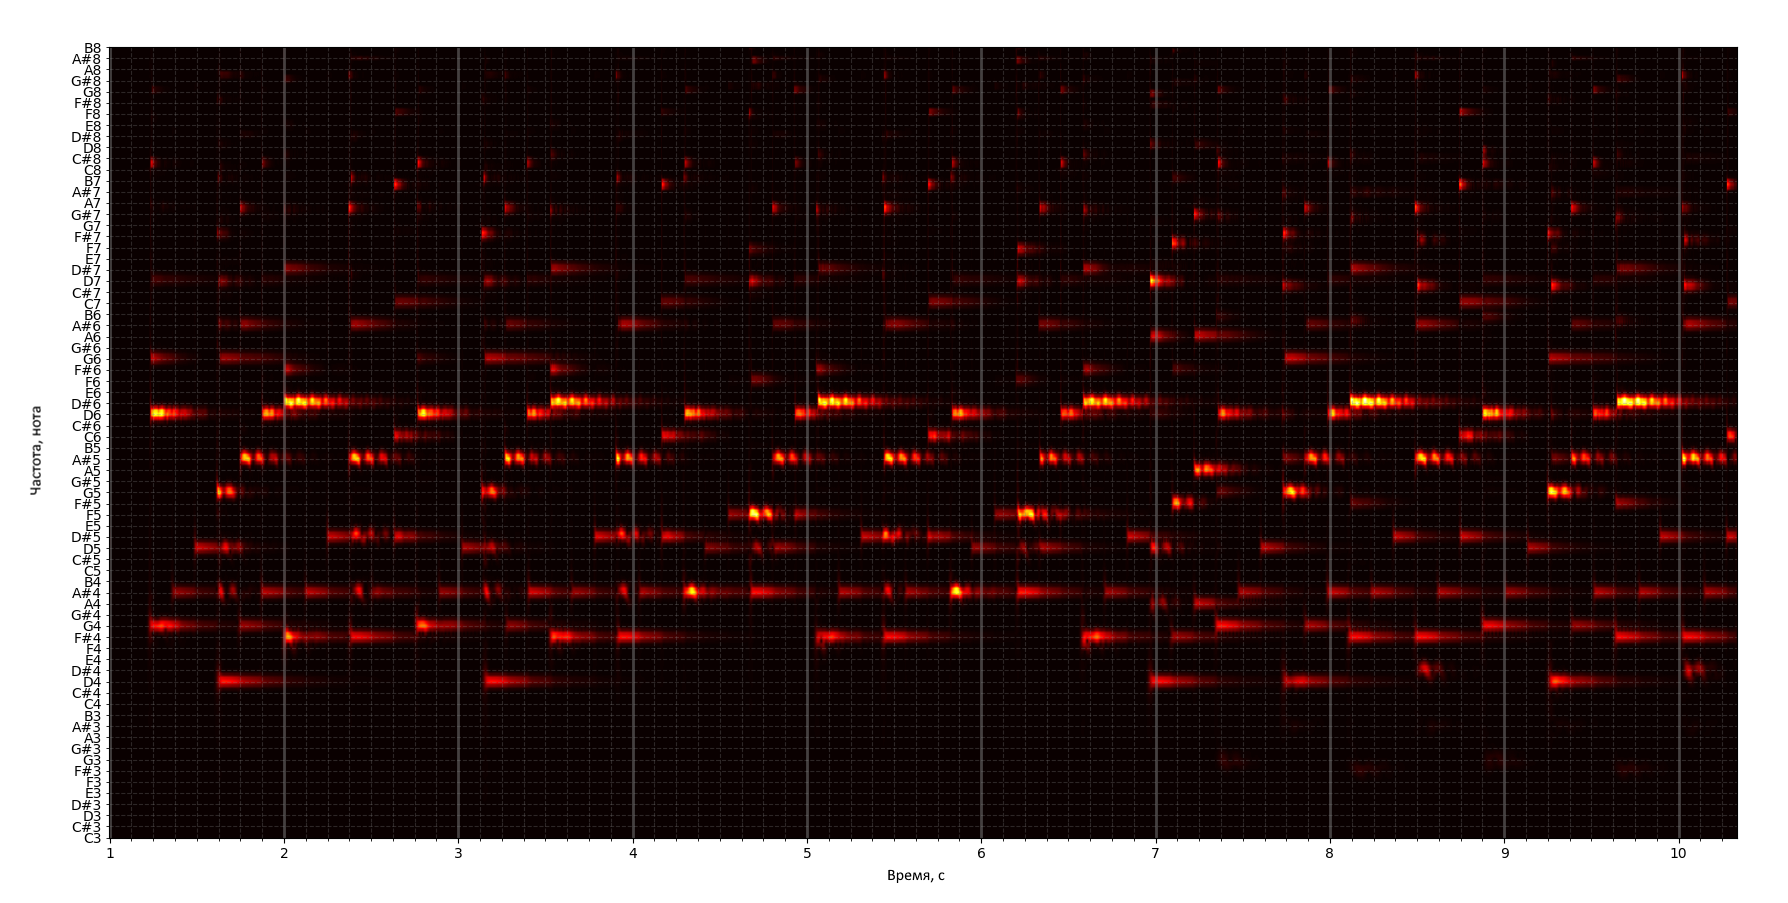
\includegraphics[width=16cm]{figures/log_spec}
  \caption{Спектрограмма записи игры на металлофоне в логарифмической шкале частот с указанием нот}
  \label{fig:log_spec}
\end{figure}

\begin{figure}[t]
  \centering
  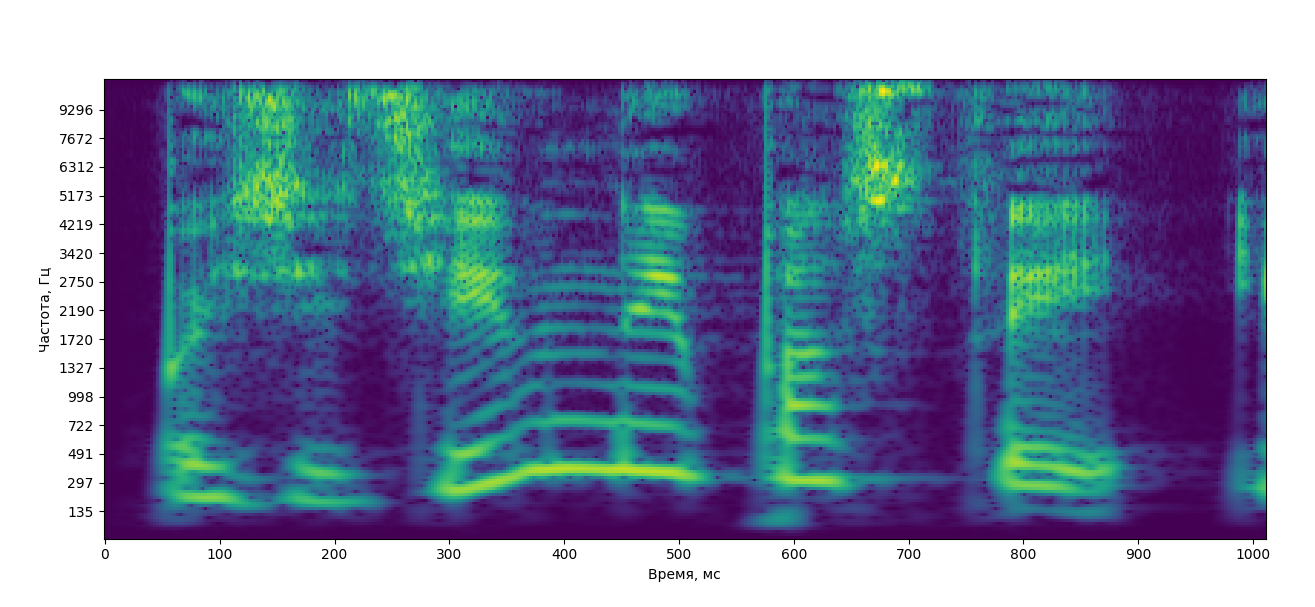
\includegraphics[width=16cm]{figures/mel_spec}
  \caption{Спектрограмма записи голоса в мел-шкале}
  \label{fig:mel_spec}
\end{figure}




\subsection{Классификация моделей}
Рассмотрим основные подходы, использующиеся в современных решениях синтеза речи и их классификацию.


\subsubsection{По формату промежуточного представления}
По формату промежуточного представления методы делятся на несколько типов:

\textbf{Генераторы спектрограмм} подразумевают генерацию спектрограммы с последующим преобразованием спектрограммы в звуковой сигнал. Примеры таких моделей:
\begin{itemize}
  \item Tacotron 2 (Google, 2017) \cite{Tacotron2} - классическая модель, использующая последовательное преобразование текста в мел-спектрограмму, с последующим применением вокодера для декодирвоания звука.
  \item FastSpeech 2 (Microsoft, 2019–2020) \cite{FastSpeech2} - Ускоренные и более стабильные версии Tacotron.
  \item Riffusion (2022) \cite{Riffusion} - Диффузионная модель, генерирующая песни и инструментальную музыку в виде спектрограмм с последующим декодированием в звук.
  \item TalkNet (2020, NVIDIA) \cite{TalkNet} - Полносверточная text-to-speech модель
\end{itemize}

\textbf{Генераторы в латентное представление} с последующим декодированием в звук с помощью нейронного декодера подразумевают 
генерацию латентного признакого представления, чем-то отдаленно схожего со спектрограммой, но сформированного отдельно обученным автоэнкодером.

\begin{itemize} 
  \item NaturalSpeech 2 (Microsoft, 2023) \cite{NaturalSpeech2} - Современная модель на основе латентных диффузий для синтеза речи и пения
  \item Kokoro-TTS (2025) \cite{kokoro}- это современная, компактная и высокоэффективная модель синтеза речи, разработанная для генерации естественного звучания при минимальных вычислительных затратах
\end{itemize}

\textbf{Генераторы токенов для нейронного кодека} схожи по принципу работы с генеративными трансформерами - основная генеративная модель создает последовательность токенов, 
которая потом преобразуется в звук с помощью нейросетевого кодека.

Пример такого кодека - EnCodec (Meta AI, 2022) \cite{encodec}. Он предназначен для сжатия и восстановления аудиосигналов, кодирует звук в дискретное латентное пространство (токены).

\begin{itemize} 
  \item Bark (Suno AI) \cite{SunoAI_Bark_2023} - Трансформерная генеративная модель, синтезирующая музыку и песни по заданному тексту и указаниям.
  \item Voicebox (2023, Meta AI) \cite{le2023voicebox} - Модель, способная генерировать, изменять и редактировать речь в различных стилях.
  \item VALL-E (Microsoft, 2023) \cite{Valle} - генерация речи с имитацией голоса на основе аудиопримера, на базе условной языковой модели.
\end{itemize}

\textbf{Одностадийные end-to-end аудиогенераторы} синтезируют звук напрямую, минуя стадию спектрограммы или отдельного декодера из латентного пространства.

\begin{itemize} 
  \item WaveNet (DeepMind, 2016) \cite{WaveNet} - Первая модель, которая напрямую генерировала звук по аудиосэмплам. Медленная, так как работает сэмпл за сэмплом (для аудио с частотой дискретизации 24 000 Гц — таких генераций должно быть 24 тысячи в секунду).
  \item DiffWave (Google, 2020) \cite{DiffWave} - Диффузионная модель, которая работает не со спектрограммой, а напрямую с аудиоволной. Высокое качество, но относительно медленная генерация.
\end{itemize}



\subsubsection{По принципу генерации промежуточного представления}
Если рассматривать принцип генерации промежуточного представления, то наиболее успешными являются трансформерные и диффузионные модели.
Также можно выделить полносверточные модели для обработки/восстановления звука, хотя существуют и полносверточные text-to-speech модели.


\textbf{Трансформерные генераторы} используют в качестве \textit{генератора} звукового представления GPT-подобный трансформер.
\begin{itemize}
  \item FastSpeech 2 (Microsoft, 2019–2020) \cite{FastSpeech2}
  \item Voicebox (2023, Meta AI) \cite{le2023voicebox}
  \item Bark (Suno AI) \cite{SunoAI_Bark_2023}
  \item Kokoro-TTS (2025) \cite{kokoro} - Поддерживает трансформеры в генераторе (настраиваемо)
  \item VALL-E (Microsoft, 2023) \cite{Valle} - генерация речи с имитацией голоса на основе аудиопримера, на базе условной языковой модели.
\end{itemize}

\textbf{Диффузионные генераторы} генерируют представление звука с помощью процесса обратной диффузии.
\begin{itemize}
  \item DiffWave (Google, 2020) \cite{DiffWave}
  \item NaturalSpeech 2 (Microsoft, 2023) \cite{NaturalSpeech2}
  \item Riffusion (2022) \cite{Riffusion}
\end{itemize}

\textbf{Полносверточные модели}
\begin{itemize} 
  \item TalkNet (2020, NVIDIA) \cite{TalkNet} - Полносверточная text-to-speech модель. В ней присутствуют отдельные полносверточные модели для предсказания длительности каждого текстового токена и модель для генерации спектрограмм. Очень быстрое обучение и синтез.
  \item Kokoro-TTS \cite{kokoro} в некоторых конфигурациях также может использовать полносверточный генератор с предсказанием длительности токенов, вместо трансформера.
  \item VoiceFixer (2022) \cite{VoiceFixer} - Восстановление повреждённой речи (например, из телефона, старых записей)
\end{itemize}


\subsection{Успехи и открытые проблемы}
Изучая успех упомянутых моделей среди сообщества и сравнивая качество синтезированного звука, можно сделать следующие выводы об успешности применения определенных технологий:

1. Существуют несколько технологий генерации звукового представления (диффузионные, трансформерные, полносверточные), способные синтезировать речь очень хорошего качества. Но такие технологии требуют больших вычислительных затрат. 
Есть оптимизированные решения, такие как Kokoro-TTS, достигающие высокого качества и высокой скорости работы за счет оптимизации архитектуры и размеров моделей, тщательной проработки и аккуратного обучения каждого компонента. 
Однако, у каждой технологии есть свои преимущества и недостатки, делающие ее более или менее пригодной для конкретной задачи.
Например: синтез музыки с множеством требований и указаний лучше всего удается диффузионным моделям. Полносверточные модели самые быстрые. 

2. Существует несколько типов вокодеров - использующие представление в виде спектрограммы, латентного представления, дискретного представления в виде токенов. Наилучшего качества в сочетании с нейросетями достигают нейросетевые вокодеры из латентного представления или спектрограммы. 
Алгоритмические вокодеры также существуют, но они неустойчивы к искажениям, которые неизбежно возникают при генерации представления с помощью нейросети, в результате чего появляются нежелательные артефакты.
Также для каждой технологии генерации подходит не любой тип промежуточного представления звука. Ниже рассмотрена совместимость технологий генерации с промежуточным представлением.

\begin{center}
\begin{tabular}{ c c c c }
                 & Спектрограмма & Латентное пр-е & Токены \\
    Диффузионные & +             & +              &        \\ 
  Трансформерные & +             & +              & +      \\  
 Полносверточные & +             & +              &     
\end{tabular}
\end{center}

Отсюда видно, что универсальными представлениями, работающими с любым типом генерации, являются спектрограмма и латентное векторное представление. 

3. Нейросетевой декодер из латентного пр-ва, обученный на одном наборе данных, 
может не подходить для применения на других данных (например на другом языке) или 
не подходить для конкретной задачи (учет интонации, акцента, персональности голоса говорящего).

4. Спектрограммные нейросетевые декодеры практически всегда требуют больших вычислительных затрат, чем из латентного пр-ва из-за избыточности информации. 
С другой стороны, в спектрограмме содержится достаточно информации для восстановления звука без потерь, 
и поэтому декодер из спектрограммы можно использовать для любой задачи, домена и технологии, и достигать наилучшего качества генерации.
Спектрограммное представление можно назвать \textit{универсальным} с точки зрения применимости технологии и задачи, но избыточным в плане вычислительных ресурсов 
(при использовании нейросетевого декодера).

5. Модели, генерирующие непосредственно звуковой сигнал, работают медленно и сложны в обучении. Практически всегда их можно разделить на две стадии - предобучение нейросетевого автоэнкодера в латентное пр-во и генерация на этом пр-ве.

6. Если бы существовал алгоритмический декодер спектрограммы, способный восстанавливать аудиосигнал с качеством, 
сопоставимым с современными нейросетевыми вокодерами, при этом устойчивый к искажениям во входных данных и обладающий более высокой скоростью работы на CPU, 
это могло бы упростить архитектуру TTS-систем, сократить вычислительные затраты и повысить доступность синтеза речи. 
Кроме того, использование стандартизированного формата спектрограмм позволило бы сосредоточить усилия на улучшении генератора, 
ускорить обучение и повысить воспроизводимость моделей.

\section{Cуществующие вокодеры}
 - Существующие Вокодеры
  - GriffinLim (algo) \cite{1164317}
  - WaveGlow (gan)
  - HiFi-Gan
  - EnCodec
  - Специализированные автоэнкодеры
 - Приемущества и недостатки существующих вокодеров 
 - примеры генерации от вокодеров, проблемы с ними
 - Алгоритм Гриффина-Лима
  - верхнеуровневое описание
 - нейросеть привязана к домену, на котором училась, алгоритм не привязан, но могут быть артефакты
 - быстродействие алгоритма и нейросети

\section{Представление и анализ аудиосигналов}
 - оконное преобразование Фурье
 - принцип неопределенности в пространстве частота-время
 - окна
 - децибел шкала амплитуд
   - почему такая
   - формула
   - порог слышимости
 - мел шкала
   - почему такая
   - формула
 - выбор оптимальной шкалы частот
  - линейная шкала
  - логарифмическая шкала
  - мел шкала
  - комбинированная шкала
 - избыточность информации в спектрограмме
 - наложение по времени
 - наложение по частоте
 - оптимальный размер окна для конкретной шкалы частот
 - сравнение с вейвлетами
 - восстановление сигнала с наложением (суммирование, сумма дает 0 там где надо, но хвосты могут расползаться)
 - оптимальная форма окна для устойчивости к искажениям
   - минимизация связанности далеких данных
 - Алгоритм Гриффина-Лима
    - как работает

 \section{Устойчивость к трансформациям и артефактам}
 - трансформации спектрограммы, устойчивость вокодера к трансформациям
   - растяжение\сжатие по времени
   - перемещение по шкале частот
   - вырезание\вставка куска
   - суммирование сигналов
 - от чего появляются трансформации и зачем нужны
 - артефакты от нейросетей
   - примеры полосок от сверток
   - BatchNorm паразитный bias
   - потеря шума
   - потеря outliers
 - устойчивость вокодеров к артефактам
 - инвариантность к сдвигу по времени, когда есть, зачем нужна

\section{Открытые проблемы}
 - борьба за качество генерации
 - как восстанавливать сигнал с нелинейной шкалой частот, когда нет ортогонального базиса
 - нет алгоритма, который был бы достаточно устойчив к артефактам от нейросетей
 - нейросетевые вокодеры:
   - требуют вычислительных ресурсов
   - нужно обучать на больших объемах данных
   - часто завязаны на домен, для другого домена могут хуже работать
 - избыточность представлений, тащим лишнюю информацию
 - нужна устойчивость обучения, глубокие сети сложнее учить

\section{Выводы по главе}

